\documentclass[11pt,graphicx,caption,rotating]{article}
\textheight=24cm
\textwidth=18cm
\topmargin=-2cm
\oddsidemargin=0cm
\usepackage[utf8x]{inputenc}
%\usepackage[latin1]{inputenc}
\usepackage[activeacute,spanish]{babel}
\usepackage{amssymb,amsfonts}
\usepackage[tbtags]{amsmath}
\usepackage{pict2e}
\usepackage{ucs}
\usepackage{float}
\usepackage[all]{xy}
\usepackage{graphics,graphicx,color,colortbl}
\usepackage{times}
\usepackage{subfigure}
\usepackage{wrapfig}
\usepackage{multicol}
\usepackage{cite}
\usepackage{url}
\usepackage[tbtags]{amsmath}
\usepackage{amsmath,amssymb,amsfonts,amsbsy}
\usepackage{bm}
\usepackage{algorithm}
\usepackage{algorithmic}
\usepackage[centerlast, small]{caption}
\usepackage[colorlinks=true, citecolor=black, linkcolor=black, urlcolor=black,breaklinks=true]{hyperref}
\hyphenation{ele-men-tos he-rra-mi-en-ta cons-tru-yen trans-fe-ren-ci-a pro-pu-es-tas si-mu-lar vi-sua-li-za-cion}

\begin{document}
\title{\textbf{Simulación en spice de una compuerta XOR utilizando la tecnología CNM25}}
\author{David Ricardo Martínez Hernández}
\date{}
\maketitle
\noindent
Inicialmente para realizar la simulación se debe construir el circuito lógico correspondiente a la compuerta XOR.\\
La tabla de verdad de esta compuerta se muestra en el Cuadro~\ref{tab1} para poder construir la función lógica:
\begin{table}[H]
  \centering
    \begin{tabular}{|c|c|c|}\hline
      $A$ & $B$ & $A XOR B$ \\ \hline
      0 & 0 & 0 \\ \hline
      0 & 1 & 1 \\ \hline
      1 & 0 & 1 \\ \hline
      1 & 1 & 0 \\ \hline
    \end{tabular}
   \caption{Tabla de verdad para la compuerta XOR.}
  \label{tab1}
\end{table}
\noindent
Se puede concluir que la función lógica se puede resimir en 
$$F = A\bar{B} + B\bar{A}$$
La función negada de la ecuación anterior se obtiene
$$\bar{F} = \overline{A \bar{B} + B \bar{A}} = (\bar{A} + B)\cdot (\bar{B} + A) $$
\noindent
Se dispone a realizar la simulación por medio de SPICE. Se debe importar la librería \textit{C5\_models.txt} la cual posee el modelo SPICE tanto para el transistor N, como para el transistor P, esta libreria fue suministrada por el profesro de laboratorio.\\
Como entradas se agregan dos señales cuadradas correspondientes a las entradas A y B.\\
En la Figura~\ref{fig2} se observan las señales, los dos primeros cuadros indican las entradas al circuito (A, B). Además el tercer cuadro se observa el resultado de la simulación, los cuales se comportaron según el Cuadro~\ref{tab1}, la salida solo está en $5\, V$ (nivel alto) cuando las entradas son diferentes, es decir una de las entradas es $0\, V$ y la otra es $5\,V$.
\begin{figure}[H]
  \centering
    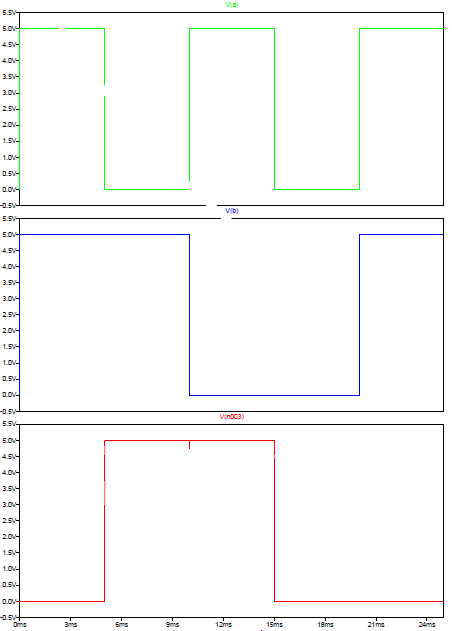
\includegraphics[scale=0.8]{fig3.png}
      \caption{Resultados de la simulación de la compuerta XOR.}
  \label{fig2}
\end{figure}
\noindent
\end{document}